% ============================================================================
%  PRL Article: Modeling Two-Dimensional Supersonic Marshak Waves
%  Uses revtex4-2 (APS journal style)
% ============================================================================
\documentclass[prl, twocolumn, superscriptaddress, amsmath, amssymb, reprint]{revtex4-2}

\usepackage{graphicx}
\usepackage{amsmath}
\usepackage{amssymb}
\usepackage{bm}
\usepackage{hyperref}
\usepackage{xcolor}
\usepackage{microtype}

\graphicspath{{figures/}}

\begin{document}

% ----------------------------------------------------------------------------
%  Title
% ----------------------------------------------------------------------------
\title{Semi-Analytic Two-Dimensional Model for Supersonic Marshak Waves in Cylindrical Geometry}

\author{Yuval Kochavi}
\affiliation{Racah Institute of Physics, The Hebrew University of Jerusalem, Jerusalem 91904, Israel}

\author{Tal Ramot}
\affiliation{Racah Institute of Physics, The Hebrew University of Jerusalem, Jerusalem 91904, Israel}

\author{Tal Balakirski}
\affiliation{Racah Institute of Physics, The Hebrew University of Jerusalem, Jerusalem 91904, Israel}

\author{Shay I.~Heizler}
\affiliation{Racah Institute of Physics, The Hebrew University of Jerusalem, Jerusalem 91904, Israel}

\date{\today}

% ----------------------------------------------------------------------------
%  Abstract
% ----------------------------------------------------------------------------
\begin{abstract}
We present, to our knowledge, the first full semi-analytic two-dimensional model for supersonic radiative Marshak-wave propagation in cylindrical foam targets. Constrained by experiment-specific drive histories and SESAME-based material fits, and compared with a few representative experiments and two-dimensional diffusion simulations, the model reproduces the main front-evolution and re-emission trends while capturing the key physical mechanisms, with wall coupling, curvature, and finite-size transport emerging as the dominant effects.
\end{abstract}

\maketitle

% ============================================================================
%  I. INTRODUCTION
% ============================================================================
% \section{Introduction}
\begingroup
\setlength{\parskip}{0pt}
\setlength{\parindent}{1em}

Radiative heat (Marshak) waves are central to high energy density physics, with direct relevance to inertial confinement fusion and astrophysical plasma analogs~\cite{Lindl2004,Rosen1996}. Modern high-power laser facilities enable controlled experiments in which hohlraum-generated x-ray drives radiation waves into low-density foams, typically surrounded by higher-$Z$ sleeves~\cite{Hinkel2006PRL}. In most cases, the heated foam is in a high-temperature, optically thick regime where both tube radius and propagation length contain several photon mean free paths, so diffusion is a good leading-order description while wall coupling remains non-negligible.

Landmark experiments by Back \textit{et al.}~\cite{Back2000PRL,Back2000POP} established diffusive, approximately supersonic x-ray transport in foam-tube targets. Subsequent campaigns extended these results to a wider range of materials, energies, sleeves, and geometries~\cite{Moore2015,Courtois2024,Keiter2008,Jiang2005,Zhang2010}. Across these studies, finite-size and wall effects emerge as leading-order controls of both front propagation and measured re-emission shape.

In this Letter, we present a compact semi-analytic framework for this class of experiments. Unified interpretation is challenging because campaigns use different drives, target designs, diagnostics, and material input models (opacity and EOS). Our framework is designed to keep physical insight while capturing the dominant multidimensional effects needed for quantitative comparison with data. Across experiments, the main differences are set by drive-temperature histories and material properties.

To anchor the discussion, Fig.~\ref{fig:setup_tdrive} summarizes the representative platform used in these supersonic x-ray transport studies: the target configuration in panel (a) and the applied drive history in panel (b)~\cite{Moore2012NIF}.
\endgroup

\begin{figure}[h!]
    \centering
    \begin{minipage}{0.5\columnwidth}
        \centering
        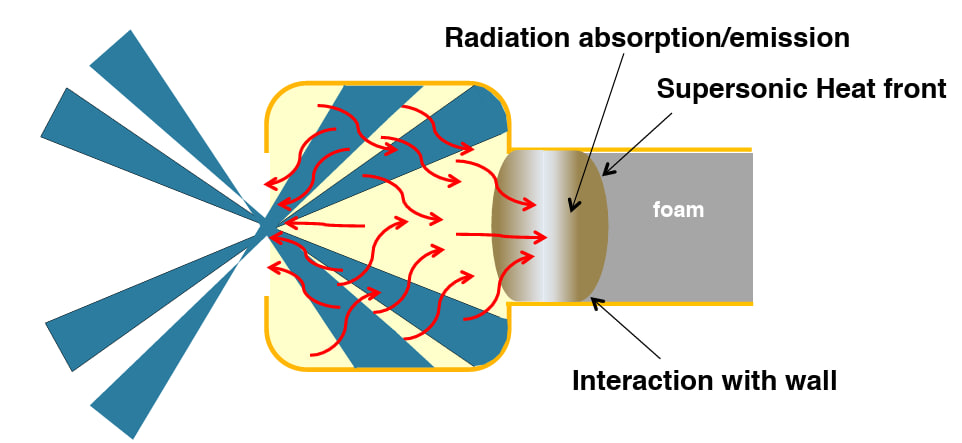
\includegraphics[width=\linewidth]{figures/setup.png}
        \vspace{-0.5em}
        \centerline{(a)}
    \end{minipage}\hfill
    \begin{minipage}{0.5\columnwidth}
        \centering
        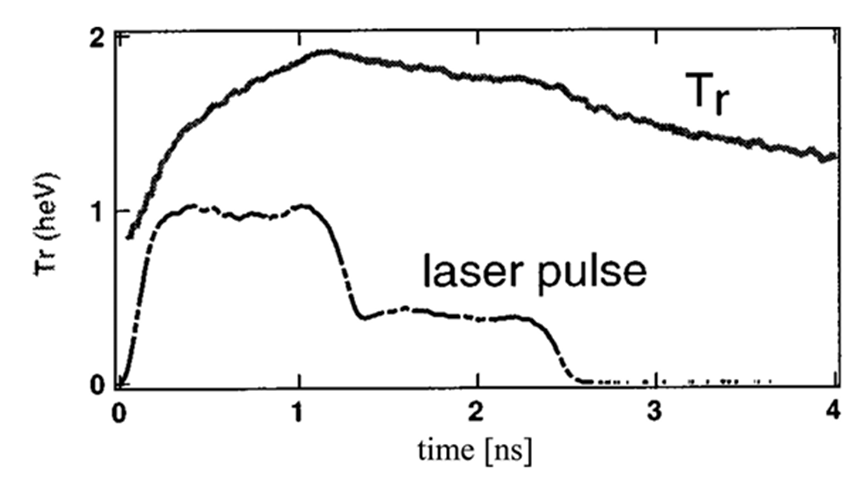
\includegraphics[width=\linewidth]{figures/T_drive.png}
        \vspace{-0.5em}
        \centerline{(b)}
    \end{minipage}
    \caption{(a) Experimental platform: laser beams enter the hohlraum through the LEH, generate x rays, and drive a Marshak wave in low-density foam targets of different lengths~\cite{Moore2012NIF}. (b) Measured hohlraum drive temperature $T_D(t)$ for the high-energy Back experiment; the dashed curve is the normalized laser pulse shape~\cite{Back2000PRL}.}
    \label{fig:setup_tdrive}
\end{figure}


% ============================================================================
%  II. GOVERNING EQUATIONS
% ============================================================================
\section{Governing Equations}

In the supersonic diffusion limit, assuming local thermodynamic equilibrium ($T_R=T_m\equiv T$), the radiation--material system reduces to a single nonlinear diffusion equation:
\begin{equation}\label{eq:diffusion}
\rho\frac{\partial e}{\partial t}
= \nabla\!\cdot\!\left(\frac{c}{3\kappa \rho}\nabla\left(aT^4\right)\right),
\end{equation}
where $a$ is the radiation constant, $c$ is the speed of light, and $\sigma = \kappa \rho$ is the Rosseland opacity.


% ============================================================================
%  III. Modeling the heat wave
% ============================================================================
\section{Modeling the Heat Wave}
In this work, we develop a semi-analytic model for supersonic Marshak-wave propagation in cylindrical geometry that extends the Hammer--Rosen one-dimensional framework~\cite{Hammer2003} to experimentally relevant finite-tube configurations. The model includes four mechanisms that control front propagation: (1) the incoming radiative flux at the foam boundary, (2) energy loss to wall heating, (3) wall ablation and the associated modification of the effective propagation channel~\cite{Cohen2020Key,Cohen2018}, and (4) finite-diameter transport effects represented through an effective MFP~\cite{Courtois2024}. We build the model in two stages: first a corrected 1D longitudinal evolution, then a 2D curvature and emission reconstruction consistent with bent-wave formulations~\cite{Hurricane2006,Courtois2022}.

We begin with the 1D Hammer--Rosen solution~\cite{Hammer2003,Rosen2009}, which assumes power laws for opacity and material energy,
$\frac{1}{\kappa}=gT^{\alpha}\rho^{-\lambda}$ and $e=fT^{\beta}\rho^{-\mu}$. Using perturbation theory, the heat-front position is
\begin{equation}\label{eq:HR}
    x_F^2(t) = \frac{2+\varepsilon}{1-\varepsilon}\,C\,H^{-\varepsilon}(t)\int_0^t H(t')\,dt',
\end{equation}
where $H(t) = T_s^{4+\alpha}(t)$, $\varepsilon = \beta/(4+\alpha)$, and
	$C = \frac{16\,g\,\sigma_{\mathrm{SB}}}{3f(4+\alpha)}\,\rho^{2-\mu-\lambda}$.
{\color{red}For each material, the material energy and opacity exponents and coefficients ($\alpha,\beta,\lambda,\mu,g,f$) are taken from fits to SESAME tables. Therefore, differences between experiments arise primarily from material property differences together with the experiment specific drive temperature reported in the corresponding references~\cite{Back2000PRL,Back2000POP,Courtois2024}.}
In this problem, it is useful to distinguish three temperatures: the drive temperature $T_D(t)$, the foam surface temperature $T_s(t)$, and the observed re-emission temperature $T_{\mathrm{obs}}(t)$. A naive assumption, $T_s(t)=T_D(t)$, gives an incorrect heat-front evolution and systematically overestimates the front velocity. For example, in our main $\mathrm{SiO}_2$ low-energy experiment~\cite{Back2000PRL}, the uncorrected HR prediction is high by about a factor of 1.5 (Fig.~\ref{fig:sio2_low_energy}).

To estimate the surface temperature $T_s(t)$, we use the Marshak boundary condition in the diffusion regime,
$\sigma_{\mathrm{SB}}T_D^4(t)=\sigma_{\mathrm{SB}}T_s^4(t)+\frac{1}{2}F(0,t)$,
which shows that $T_s(t)$ is set by the boundary flux $F(0,t)$. The HR framework also provides the stored material energy,
$E(t)=f\rho^{1-\mu}x_F(t)H^{\varepsilon}(t)(1-\varepsilon)$, with $\dot{E}(t)=F(0,t)$ at the boundary. Solving these relations together with Eq.~(\ref{eq:HR}) yields a physics-based $T_s(t)$ and reduces reliance on ad hoc temperature-reduction factors.

We now extend the model to 2D effects. A primary source of front retardation in cylindrical-tube experiments is radiative energy loss into the surrounding walls. As the heat wave propagates along the axis, each axial slice of foam is exposed to radiation from its local front-arrival time $t_0(x)$. The wall at that position then absorbs energy for the remaining duration $t-t_0(x)$. {\color{red}We evaluate the cumulative wall-deposited energy using the cylindrical wall-loss integral form and material-dependent self-similar wall-heating laws reported in Refs.~\cite{Cohen2020Key,Cohen2018}. For gold walls we use the corresponding subsonic scaling from those same references.}
Wall losses reduce the energy retained by the foam and therefore slow the front (Fig.~\ref{fig:sio2_low_energy}). {\color{red}Analogous expressions, with different coefficients, apply to other coating materials such as beryllium or copper.}

Beyond direct energy removal, the heated wall ablates inward, reducing the effective tube radius over time. This ablation effect is relevant only for high-$Z$ and mid-$Z$ sleeve materials, which are subsonic in the relevant temperatures --- in our experiments, gold and copper --- whereas for low-$Z$ beryllium or vacuum sleeves, the ablation is negligible, and the effect is omitted. {\color{red}The ablation-velocity law, including its density-dependent prefactor, is taken from the self-similar subsonic treatment of Ref.~\cite{Cohen2020Key}. The tube radius is then updated in time, and the incoming energy is evaluated through the corresponding reduced-area integral following Refs.~\cite{Cohen2020Key,Cohen2018}.}
In addition, the ablated material compresses the foam, raising the mean density $\rho(t) = \rho_0 V_0 / V(t)$ where $V(t) =  \int_0^{x_F(t)}\pi R^2(t,x)\,dx$. This retards the front further, making the HR coefficient time dependent through a density-history integral~\cite{Cohen2020Key,Cohen2018}. Together, wall-energy loss and ablation-driven compression are the dominant 2D corrections that bring the model into quantitative agreement with experiment (Fig.~\ref{fig:sio2_low_energy}).

A further correction arises when the Rosseland MFP $\lambda_R = 1/(\kappa\rho)$ becomes comparable to or larger than the tube diameter $2R$. In that regime photon transport is no longer governed by absorbtions and emmisions but is increasingly limited by wall collisions, reducing the effective MFP below the diameter value. Following Ref.~\cite{Courtois2024}, we account for this by replacing $\lambda_R$ with
 $\lambda_{\mathrm{eff}} = \left[\left(2R\right)^{-n} + \lambda_R^{-n}\right]^{-1/n}$,
where $n$ controls the sharpness of the transition. In the diffusion limit such as in the SiO$_2$ low energy~\cite{Back2000PRL} ($\lambda_R \ll 2R$), $\lambda_{\mathrm{eff}} \to \lambda_R$, and so the effect is quite neglectable. In the wall-collision limit ($\lambda_R \gg 2R$), $\lambda_{\mathrm{eff}} \to 2R$. This correction is most significant in optically thin, low-density foams where $\lambda_R$ is large: the tube diameter becomes the transport bottleneck, yielding an effective diffusivity below the bulk Rosseland value. The effect is included in the model through the time-dependent $\lambda_{\mathrm{eff}}(t)$, which modifies the HR coefficient $C(t) = \frac{16\,g\,\sigma_{\mathrm{SB}}}{3f(4+\alpha)t}\,\rho^{2-\mu-\lambda}\,\int_{0}^{t}\lambda_{\mathrm{eff}}(t')dt'$ and hence the front evolution.

\begin{figure}[h!]
	\centering
	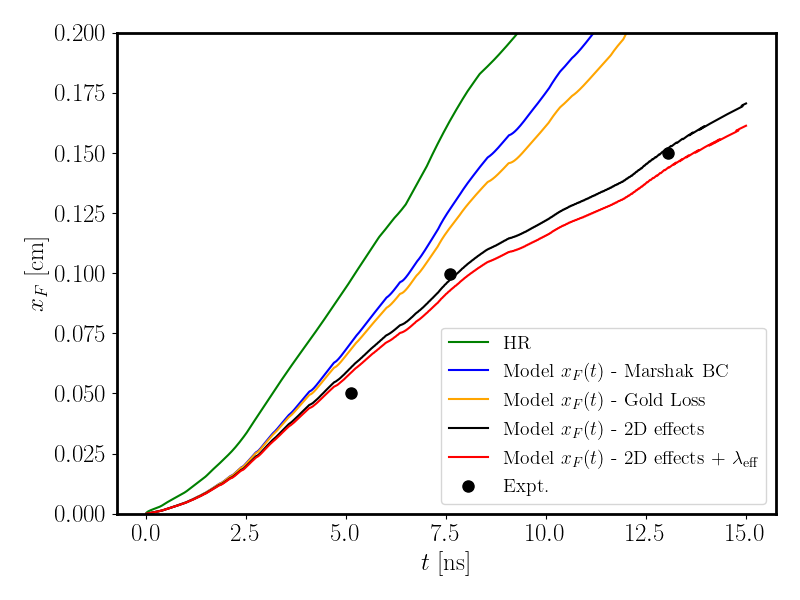
\includegraphics[width=\columnwidth]{figures/SiO2_low_energy.png}
	\caption{Front-position comparison for the $\mathrm{SiO}_2$ low-energy case, illustrating the effect of the corrected 1D and 2D terms.}
	\label{fig:sio2_low_energy}
\end{figure}

The 1D front position $x_F(t)$ captures only axial propagation, whereas the physical front is curved, primarily by radiative losses to the sleeve. This curvature is experimentally important because the measured signal is the re-emission intensity, $\Phi\propto T^4$, which strongly amplifies transverse temperature variations. As a result, the intrinsically 2D front shape both delays breakout at the diagnostic plane and feeds back on the energy balance, since wall losses are controlled by the boundary-front evolution at $r=R$.

To describe this curvature quantitatively, Hurricane and Hammer~\cite{Hurricane2006} showed that, in the idealized limit of constant opacity, negligible material-energy storage, and a steep heat front, the hot region behind the front is governed by a Laplace problem. In that formulation, the lossy wall enters through a Robin boundary condition set by the wall albedo {\color{red}(see the Appendix)}: only a fraction $\alpha$ of the incident radiative flux is returned to the foam, while $1-\alpha$ is absorbed by the surrounding wall. This partial return cools the tube edge relative to the axis, and the resulting transverse eigenmodes bend the front. For a planar channel these modes are cosines, while in an axisymmetric cylindrical tube the regular radial modes are zeroth-order Bessel modes $J_0$ due to symmetry at $r=0$. The cylindrical analogue therefore has the leading-order form~\cite{Courtois2022}
\begin{equation}\label{eq:HH_cyl}
    x_F(r,t) = \frac{1}{\kappa_0}\cosh^{-1}\!\left(1 + \frac{D\kappa_0^2 t}{2}\right)J_0(\kappa_0 r) + \text{H.O.T.}
\end{equation}
The transverse wavenumber is fixed by the wall-loss boundary condition. In the weak-loss, high-albedo limit, $\kappa_0 \approx \sqrt{2\varepsilon}/R$ with $\varepsilon = \tfrac{3}{4}\rho\kappa R(1-\alpha)$ and $\alpha$ the wall albedo {\color{red}(see the Appendix)}. This approximation is accurate for small $\varepsilon$, i.e., $\alpha\to1$. However, in relevant lower-albedo cases (e.g., copper with $\alpha\sim0.5$ and beryllium with $\alpha\sim0.3$), the small-$\varepsilon$ expansion is no longer sufficiently accurate. In those cases we compute $\kappa_0$ from a numerical solution of the transverse eigenvalue problem with the full wall-loss boundary condition {\color{red}(see the Appendix)}. Thus $J_0(\kappa_0 r)$ describes the curvature, while the coefficient multiplying it describes the longitudinal advance of the front.

The key remaining quantity that sets the curvature is the wall albedo. Instead of prescribing a constant fitted value~\cite{Hurricane2006,Courtois2022}, we compute a time-dependent $\alpha(t)=F_{\mathrm{out}}/F_{\mathrm{in}}$ from the local interface energy balance between incoming radiative flux, re-emitted flux, and absorbed wall energy. {\color{red}The explicit expression is given in the Appendix.}
This gives $\varepsilon(t)=\tfrac{3}{4}\rho\kappa R\,[1-\alpha(t)]$, and therefore a time-dependent $\kappa_0(t)$ and front curvature. Stronger wall absorption lowers $\alpha(t)$, increases $\kappa_0(t)$, and yields a more strongly curved front. In the high-albedo limit $\alpha\to1$, $\kappa_0\to0$, and the model recovers the one-dimensional limit. Meaning gold sleeves produce an almost flat front, while beryllium sleeves, produce a more pronounced curvature.
Opacity also evolves in time through $T(t)$ and directly affects front curvature, this dependence is already included through the power-law closure $\kappa^{-1}=gT^{\alpha}\rho^{-\lambda}$ used in the model.

With this dynamic-albedo closure, we retain the separation of variables form only for the transverse structure and replace the longitudinal factor in Eq.~(\ref{eq:HH_cyl}) by the corrected centerline evolution from the longitudinal model. The resulting front model, $x_F(r,t)=x_F(t)J_0\!\left(\kappa_0 r\right)$, is then compared with 2D diffusion simulations without hydrodynamics:

\begin{figure}[h!]
	\centering
	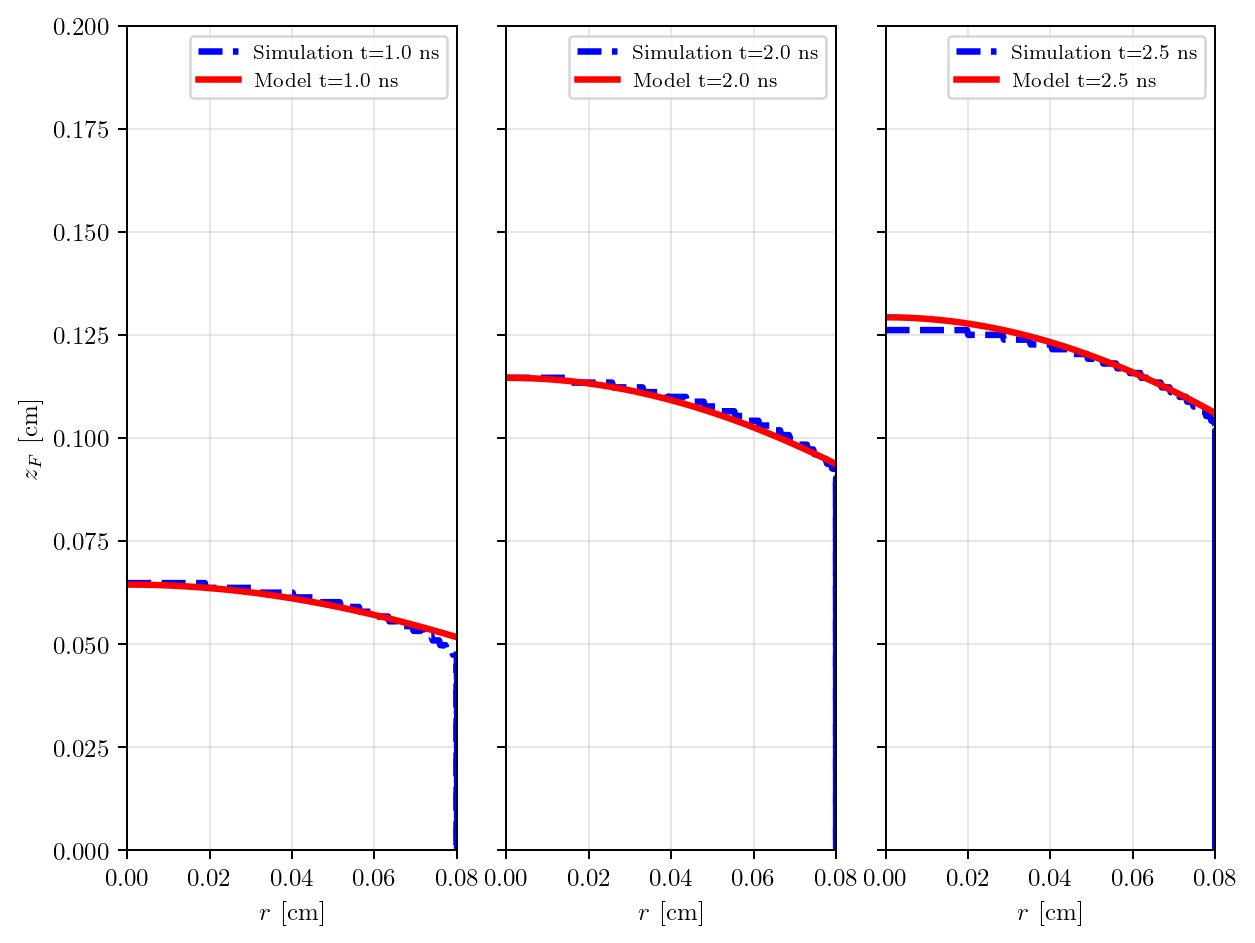
\includegraphics[width=0.9\columnwidth]{figures/front_surface_gold100.png}
	\caption{{\color{red}2D front comparison for the low-energy $\mathrm{SiO}_2$ case~\cite{Back2000PRL} with different coatings: Au, Cu, Be, and vacuum. The model agrees well with simulation, and the wall-material effect is clearly visible.}}
	\label{fig:simulation_comparison}
\end{figure}


Once the curved front is known, we reconstruct the two-dimensional temperature field by combining the corrected longitudinal temperature profile with the radial eigenmode structure. The front shape determines which axial positions have been heated at each radius, while the itiiolocal temperature behind the front follows the Henyey-like profile used in the one-dimensional solution~\cite{Hammer2003,Rosen2009}, with radial dependece through the front position,
\begin{equation}\label{eq:henyey_profile}
T(r,x,t) = T_s(t)\left[1-\dfrac{x}{x_F(r,t)}\right]^{\frac{1}{4+\alpha-\beta}}
\end{equation}
where $x_F(r,t)$ is the curved heat-front position and $T_s(t)$ is the surface temperature obtained from the corrected 1D Marshak calculation. This gives a map of $T^4(r,x,t)$, shown in Fig.~\ref{fig:temperature_flux_curvature}(a), from which the observable re-emission pattern is computed directly. At a diagnostic plane $x=x_{\mathrm{det}}$, the model flux curvature is $\Phi(r,x_{\mathrm{det}},t)=\sigma_{\mathrm{SB}}T^4(r,x_{\mathrm{det}},t)$,
and the resulting radial profile is normalized to its peak before comparison with the measured emission profile. The same wall-loss eigenmode that bends the heat front therefore also produces the depressed edge emission seen in Fig.~\ref{fig:temperature_flux_curvature}(b).

Figure~\ref{fig:temperature_flux_curvature}(c) shows an additional experimental curvature dataset from Back \textit{et al.}~\cite{Back2000POP} for Ta$_2$O$_5$, evaluated at the temporal peak of the emitted x-ray signal (0.5 ns after breakout). The samples are 0.25, 0.50, 0.75, and 1.00 mm long: the shorter samples (0.25 and 0.50 mm) are exposed to heating for a longer time, are therefore more diffusive, and are reproduced more accurately by the model. For the longer samples (0.75 and 1.00 mm), the diffusion approximation is less valid, and the agreement is correspondingly worse. This comparison highlights both the predictive strength and the validity limits of the diffusion-based model.

\begin{figure*}[t]
    \centering
    \begin{minipage}{0.38\textwidth}
        \centering
        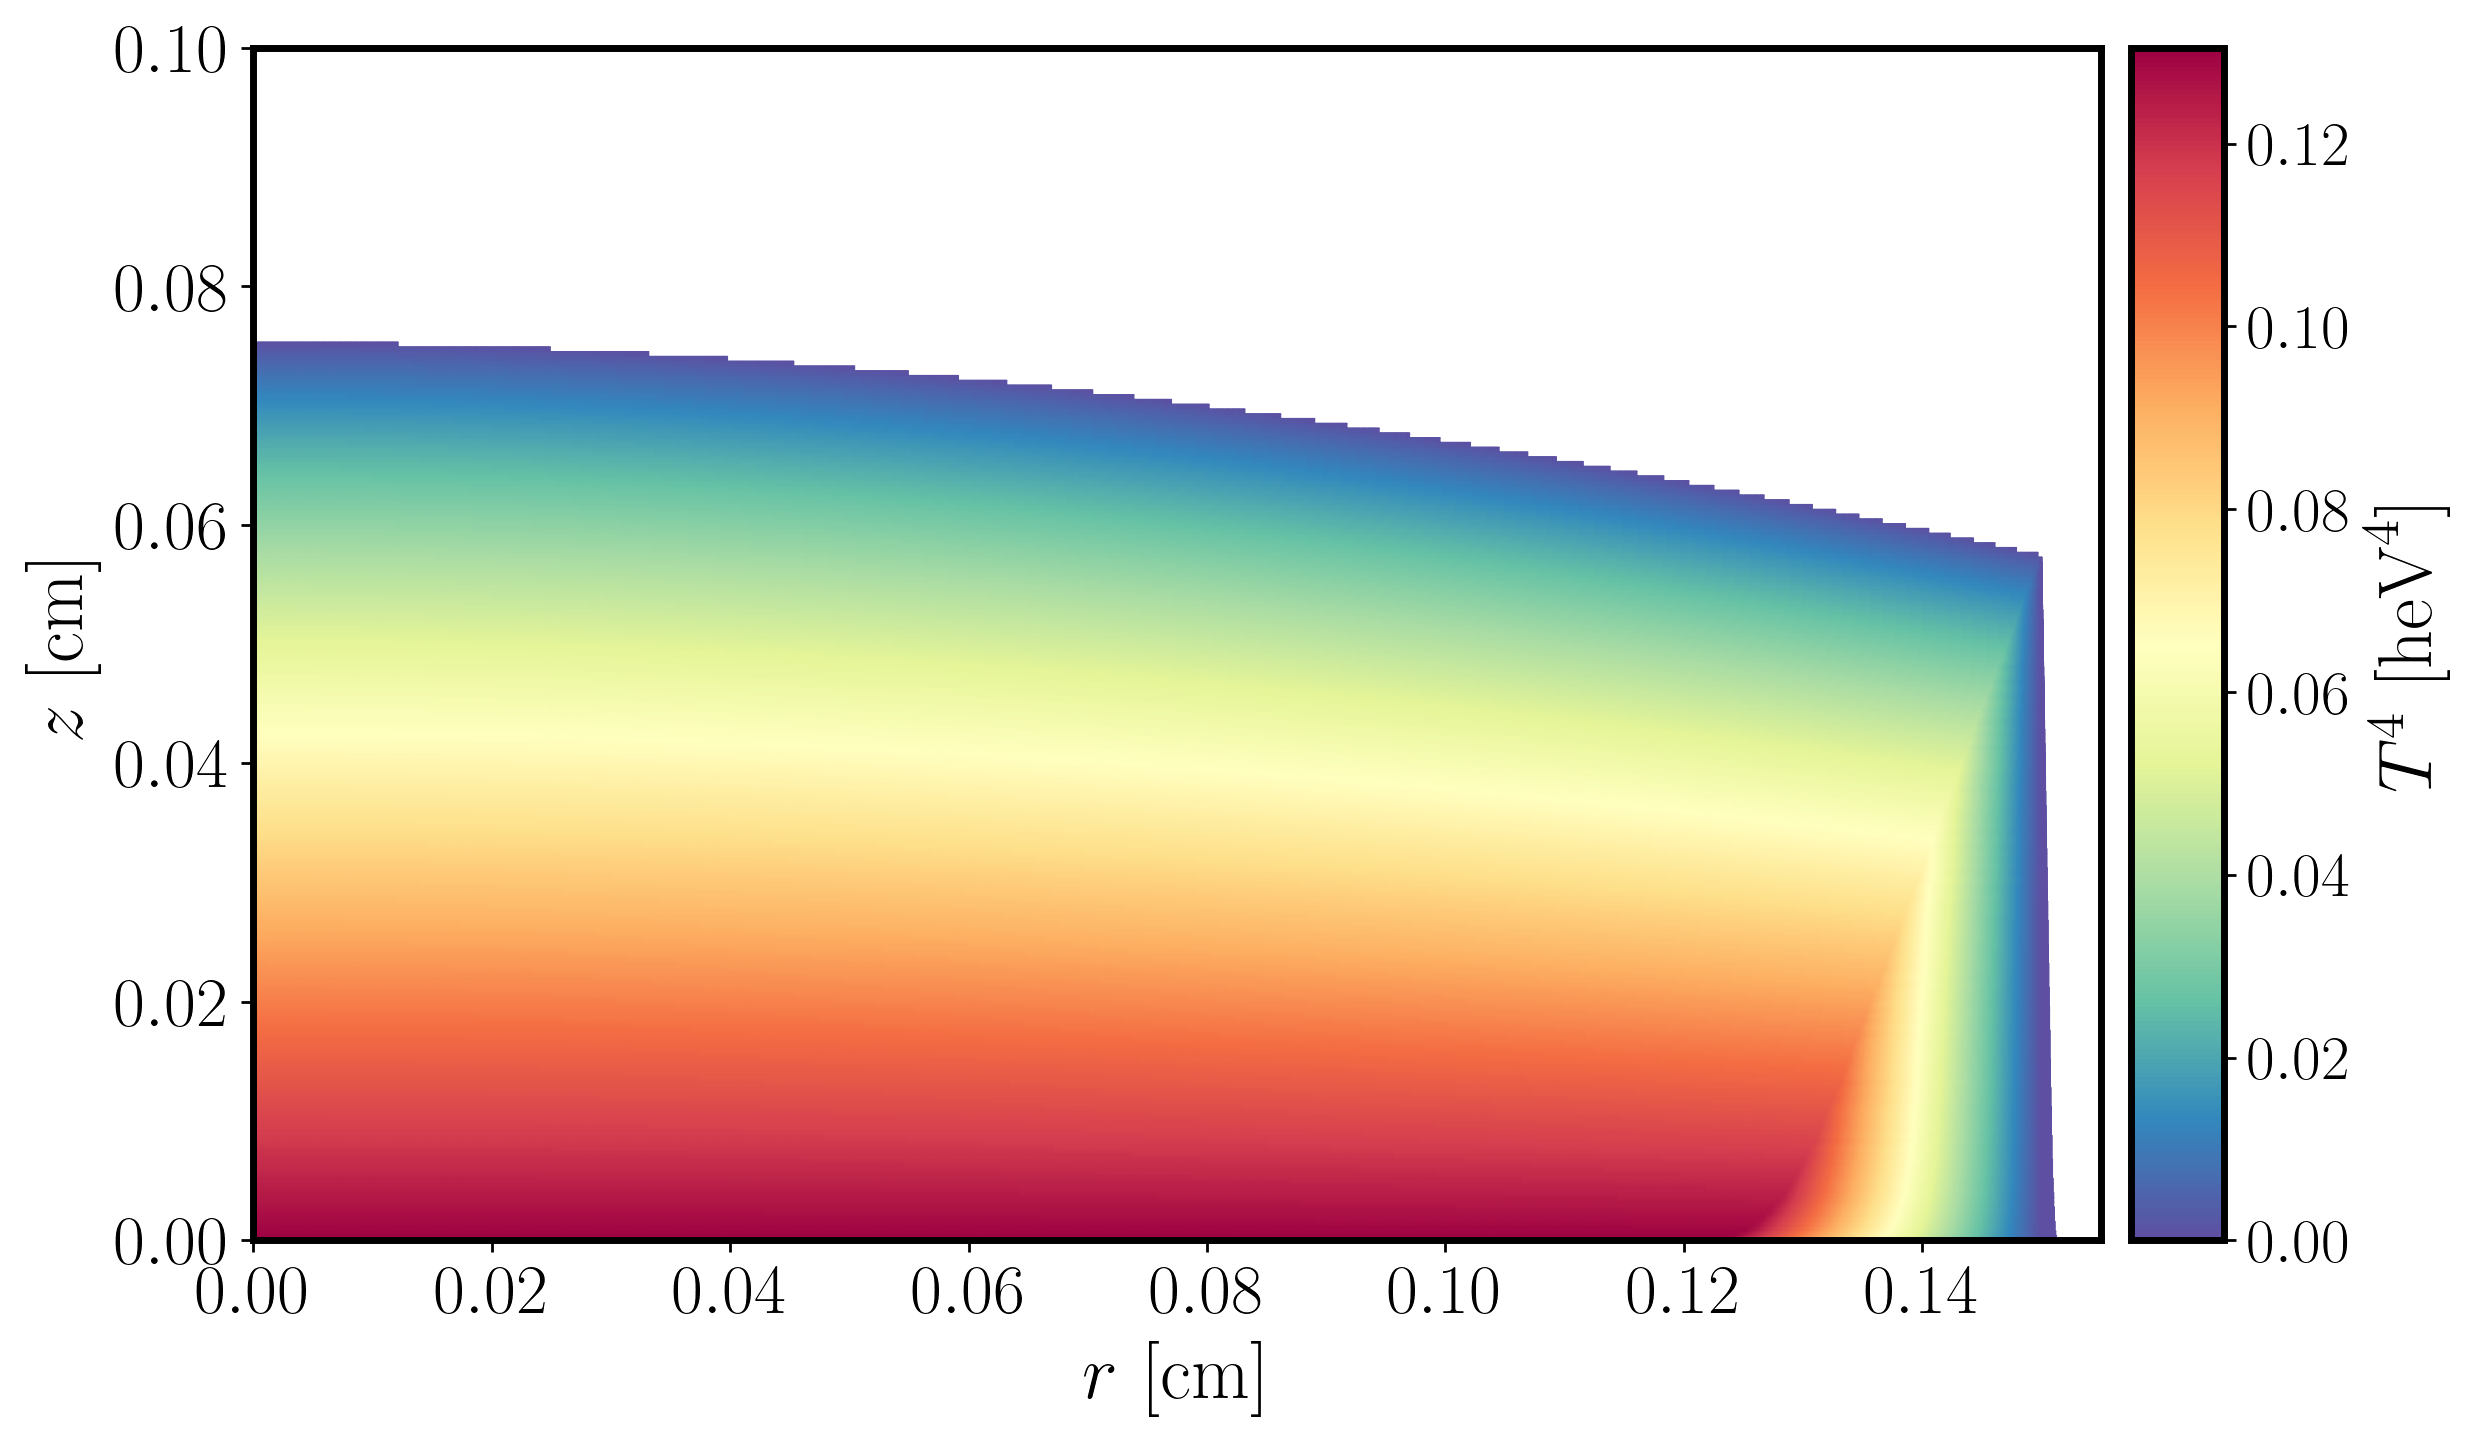
\includegraphics[width=\linewidth]{figures/prl_T4.png}
        \vspace{-0.8em}
        \centerline{(a)}
    \end{minipage}\hfill
    \begin{minipage}{0.28\textwidth}
        \centering
        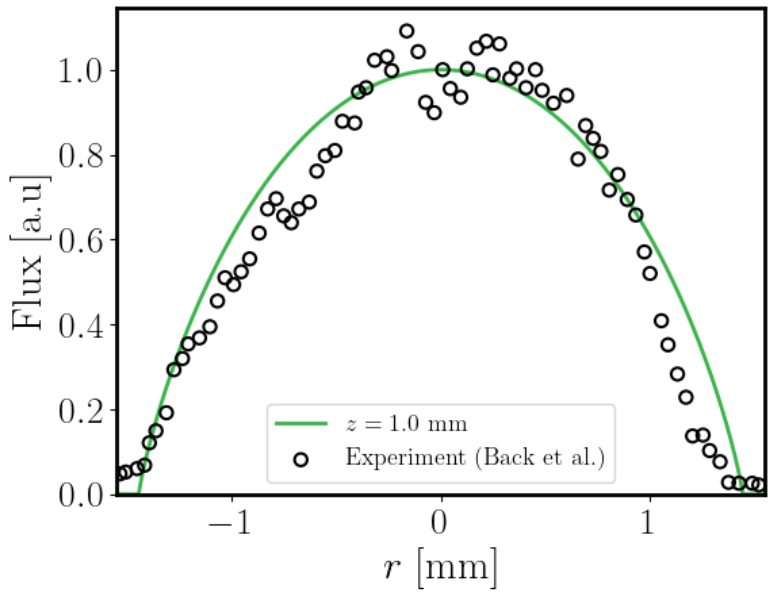
\includegraphics[width=\linewidth]{figures/back_prl_curve.png}
        \vspace{-0.8em}
        \centerline{(b)}
    \end{minipage}\hfill
    \begin{minipage}{0.3\textwidth}
        \centering
        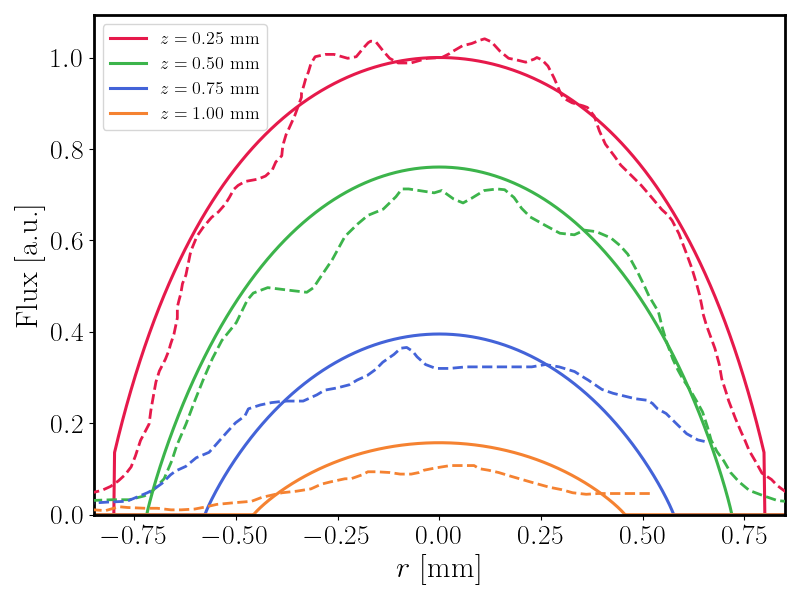
\includegraphics[width=\linewidth]{figures/back_pop_ta2o5_curve.png}
        \vspace{-0.8em}
        \centerline{(c)}
    \end{minipage}
    \caption{Temperature reconstruction and flux curvature. (a) Two-dimensional $T^4(r,z)$ profile obtained by the model at time 6 ns. (b) A cross section of the radial flux profile, compared with the Back \textit{et al.} radial intensity data. (c) Additional experimental flux-curvature comparison for Ta$_2$O$_5$ from Back \textit{et al.}~\cite{Back2000POP}, taken at the temporal peak of the emitted x-ray signal (0.5 ns after breakout).}
    \label{fig:temperature_flux_curvature}
\end{figure*}


% ============================================================================
%  V. CONCLUSION
% ============================================================================
\section{Conclusion}

We presented a compact semi-analytic framework for supersonic Marshak-wave propagation in cylindrical geometries, formulated to preserve physical insight while capturing the leading multidimensional effects that shape experimental observables. In this sense, the model provides a practical middle ground between idealized analytic descriptions and fully numerical simulations.

Across the benchmark cases examined here, the framework reproduces the main trends in front evolution and re-emission curvature, including clear material dependence. The largest deviations appear where the underlying diffusion assumptions become less accurate, which also clarifies the model's domain of validity. Overall, this approach offers a fast and interpretable tool for experiment analysis and design, and a flexible basis for future extensions to broader transport regimes.



% ============================================================================
%  REFERENCES
% ============================================================================
\begin{thebibliography}{99}

\bibitem{Lindl2004}
J.~D.~Lindl, P.~Amendt, R.~L.~Berger, S.~G.~Glendinning, and S.~H.~Glenzer,
Phys.\ Plasmas \textbf{11}, 339 (2004).

\bibitem{Rosen1996}
M.~D.~Rosen,
Phys.\ Plasmas \textbf{3}, 1803 (1996).

\bibitem{Hammer2003}
J.~H.~Hammer and M.~D.~Rosen,
\textit{A consistent approach to solving the radiation diffusion equation},
Phys.\ Plasmas \textbf{10}, 1829 (2003).

\bibitem{Rosen2009}
M.~D.~Rosen,
\textit{Lectures in the Scottish Universities Summer School in Physics, 2005, on High Energy Laser Matter Interactions},
in \textit{High Energy Laser Matter Interactions}, edited by D.~A.~Jaroszynski, R.~Bingham, and R.~A.~Cairns
(CRC Press, Boca Raton, 2009), p.~325.

\bibitem{Shussman2015}
T.~Shussman and S.~I.~Heizler,
\textit{Full self-similar solutions of the subsonic radiative heat equations},
Phys.\ Plasmas \textbf{22}, 082109 (2015).

\bibitem{Pomraning1979}
G.~C.~Pomraning,
\textit{The Equations of Radiation Hydrodynamics}
(Pergamon, Oxford, 1973).

\bibitem{Back2000PRL}
C.~A.~Back, J.~D.~Bauer, J.~H.~Hammer \textit{et al.},
\textit{Diffusive, supersonic x-ray transport in radiatively heated foam cylinders},
Phys.\ Rev.\ Lett.\ \textbf{84}, 274 (2000).

\bibitem{Hinkel2006PRL}
D.~E.~Hinkel, M.~B.~Schneider, B.~K.~Young, A.~B.~Langdon, E.~A.~Williams, M.~D.~Rosen, and L.~J.~Suter,
\textit{Creation of hot radiation environments in laser-driven targets},
Phys.\ Rev.\ Lett.\ \textbf{96}, 195001 (2006).

\bibitem{Back2000POP}
C.~A.~Back, J.~D.~Bauer, O.~L.~Landen \textit{et al.},
\textit{Detailed measurements of a diffusive supersonic wave in a radiatively heated foam},
Phys.\ Plasmas \textbf{7}, 2126 (2000).

\bibitem{Moore2015}
A.~S.~Moore, T.~M.~Guymer, J.~Morton \textit{et al.},
\textit{Characterization of supersonic radiation diffusion waves},
J.\ Quant.\ Spectrosc.\ Radiat.\ Transfer \textbf{159}, 100 (2015).

\bibitem{Keiter2008}
P.~Keiter, M.~Gunderson, J.~Foster \textit{et al.},
\textit{Radiation transport in inhomogeneous media},
Phys.\ Plasmas \textbf{15}, 056901 (2008).

\bibitem{Jiang2005}
S.~Jiang, Y.~Xu, Y.~Ding \textit{et al.},
\textit{Experimental investigation of supersonic radiation propagation in low-density plastic and copper-doped foams},
Sci.\ China Ser.\ G \textbf{48}, 549 (2005).

\bibitem{Zhang2010}
J.-Y.~Zhang, J.-M.~Yang, S.-E.~Jiang \textit{et al.},
\textit{Experimental observation of ionization and shock fronts in foam targets driven by thermal radiation},
Chin.\ Phys.\ B \textbf{19}, 025201 (2010).

\bibitem{Moore2012NIF}
A.~S.~Moore, J.~L.~Kline, P.~A.~Keiter, J.~Morton, T.~M.~Guymer,
G.~Magelssen, B.~Devolder, K.~A.~Mussack, R.~Peterson, J.~M.~Taccetti,
N.~Lanier, M.~Stevenson, J.~Workman, K.~A.~Obrey, D.~Schmidt,
C.~Hamilton, D.~Capelli, J.~Williams, B.~Randolph, F.~Fierro,
J.~Martinez, B.~Patterson, N.~Bazin, and S.~Goodinga,
\textit{NIF presentation} (2012).

\bibitem{Cohen2018}
A.~P.~Cohen and S.~I.~Heizler,
J.\ Comput.\ Theor.\ Transp.\ \textbf{47}, 378 (2018).

\bibitem{Cohen2020Key}
A.~P.~Cohen, G.~Malamud, and S.~I.~Heizler,
\textit{Key to understanding supersonic radiative Marshak waves using simple models and advanced simulations},
Phys.\ Rev.\ Research \textbf{2}, 023007 (2020).

\bibitem{Hurricane2006}
O.~A.~Hurricane and J.~H.~Hammer,
\textit{Bent Marshak waves},
Phys.\ Plasmas \textbf{13}, 113303 (2006).

\bibitem{Courtois2022}
C.~Courtois, R.~Gr\"oger, P.~Loiseau \textit{et al.},
\textit{Models for the propagation of radiation heat fronts in cylindrical tubes},
Phys.\ Plasmas \textbf{29}, 022704 (2022).

\bibitem{Courtois2024}
C.~Courtois, R.~Gr\"oger, P.~Loiseau \textit{et al.},
\textit{Experimental measurements of supersonic radiation heat wave curvature in cylindrical tubes},
Phys.\ Plasmas \textbf{31}, 012707 (2024).

\end{thebibliography}

\end{document}
